\documentclass[UTF8,11pt,a4paper,fontset=none]{ctexart}
\setCJKmainfont[AutoFakeBold=true]{Songti SC}
\setCJKsansfont[AutoFakeBold=true]{Heiti SC}
\setCJKmonofont{Songti SC}
\usepackage[left=24mm,right=24mm,top=25mm,bottom=25mm]{geometry}
\usepackage{amsmath,amssymb,mathtools,booktabs,array,graphicx}
\usepackage{xcolor,hyperref,fancyhdr,listings}
\usepackage[most]{tcolorbox}
\definecolor{deepblue}{RGB}{36,55,122}
\definecolor{keyred}{RGB}{162,30,37}
\definecolor{pale}{RGB}{241,244,251}
\hypersetup{colorlinks=true,linkcolor=deepblue,urlcolor=deepblue}
\ctexset{section={format=\Large\bfseries\color{deepblue}},
 subsection={format=\large\bfseries\color{deepblue}}}
\pagestyle{fancy}
\fancyhf{}
\fancyhead[L]{MATH4907 Tutorial 5}
\fancyhead[R]{Assignment 5 逐题讲解}
\fancyfoot[C]{\thepage}
\renewcommand{\headrulewidth}{0.3pt}
\setlength{\headheight}{14pt}
\newcommand{\E}{\mathbb E}
\newcommand{\Var}{\operatorname{Var}}
\newcommand{\Cov}{\operatorname{Cov}}
\newcommand{\SE}{\operatorname{SE}}
\newtcolorbox{idea}{colback=pale,colframe=deepblue!65!white,
 boxrule=0.5pt,arc=1mm,left=2mm,right=2mm,top=1mm,bottom=1mm}
\newtcolorbox{pitfall}{colback=keyred!4!white,colframe=keyred!65!white,
 boxrule=0.5pt,arc=1mm,left=2mm,right=2mm,top=1mm,bottom=1mm}
\lstset{basicstyle=\ttfamily\small,columns=fullflexible,keepspaces=true,
 frame=single,backgroundcolor=\color{pale},showstringspaces=false}
\graphicspath{{figures/}}
\newcommand{\QOneStates}{6, 13, 14, 5, 6, 13, 14, 5, 6, 13, 14, 5, 6, 13, 14, 5, 6, 13, 14, 5}
\newcommand{\QOneUniforms}{0.3750, 0.8125, 0.8750, 0.3125, 0.3750, 0.8125, 0.8750, 0.3125, 0.3750, 0.8125, 0.8750, 0.3125, 0.3750, 0.8125, 0.8750, 0.3125, 0.3750, 0.8125, 0.8750, 0.3125}
\newcommand{\QTwoMean}{2.029487}
\newcommand{\QTwoVariance}{4.074184}
\newcommand{\QThreeProposals}{15100}
\newcommand{\QThreeEfficiency}{0.662252}
\newcommand{\QFourExact}{0.746824133}
\newcommand{\QFourAMean}{0.747220}
\newcommand{\QFourASD}{0.197787}
\newcommand{\QFourALow}{0.708454}
\newcommand{\QFourAHigh}{0.785986}
\newcommand{\QFourBMean}{0.746617}
\newcommand{\QFourBSD}{0.201933}
\newcommand{\QFourBLow}{0.734101}
\newcommand{\QFourBHigh}{0.759133}
\newcommand{\QFourCMean}{0.743719}
\newcommand{\QFourCSD}{0.201024}
\newcommand{\QFourCLow}{0.739779}
\newcommand{\QFourCHigh}{0.747659}
\newcommand{\QFourDMean}{0.746570}
\newcommand{\QFourDSD}{0.200986}
\newcommand{\QFourDLow}{0.745324}
\newcommand{\QFourDHigh}{0.747816}
\newcommand{\QFiveExact}{13.455050}
\newcommand{\QFiveAMean}{13.267172}
\newcommand{\QFiveASD}{26.497851}
\newcommand{\QFiveASE}{0.264979}
\newcommand{\QFiveALow}{12.747814}
\newcommand{\QFiveAHigh}{13.786529}
\newcommand{\QFiveBMean}{13.439328}
\newcommand{\QFiveBSD}{27.220361}
\newcommand{\QFiveBSE}{0.086078}
\newcommand{\QFiveBLow}{13.270615}
\newcommand{\QFiveBHigh}{13.608042}
\newcommand{\QSixAVMean}{13.646271}
\newcommand{\QSixAVSD}{16.678473}
\newcommand{\QSixAVSE}{0.166785}
\newcommand{\QSixAVLow}{13.319373}
\newcommand{\QSixAVHigh}{13.973169}
\newcommand{\QSixCrudeMean}{13.603578}
\newcommand{\QSixCrudeSD}{27.161508}
\newcommand{\QSixCrudeSE}{0.271615}
\newcommand{\QSixCrudeLow}{13.071212}
\newcommand{\QSixCrudeHigh}{14.135943}
\newcommand{\QSevenCoeff}{-0.863741}
\newcommand{\QSevenExact}{0.961766}
\newcommand{\QSevenExactCoeff}{-0.865589}
\newcommand{\QSevenCrudeMean}{0.985239}
\newcommand{\QSevenCrudeSD}{0.884294}
\newcommand{\QSevenCrudeSE}{0.008843}
\newcommand{\QSevenCVMean}{0.962008}
\newcommand{\QSevenCVSD}{0.048498}
\newcommand{\QSevenCVSE}{0.000485}

\begin{document}

\begin{center}
{\huge\bfseries\color{deepblue} MATH4907 Tutorial 5}\\[3mm]
{\Large Assignment 5：蒙特卡洛方法逐题讲解}\\[5mm]
Sanyang Liu \qquad 2026 年 11 月 20 日
\end{center}
\vspace{3mm}
\begin{idea}
本讲义按七道题及各小问顺序展开。数值结果来自固定随机种子的模拟；换用别的种子，数值可以不同，推导、算法和统计量的定义应相同。同目录的 \texttt{05\_tutorial.py} 可复现结果与图。
\end{idea}
\tableofcontents
\newpage

\section{先建立贯穿七题的思路}
蒙特卡洛方法先把目标写为期望 $\theta=\E[H(X)]$，再从 $X$ 的分布独立抽取 $X_1,\ldots,X_N$，用
\begin{equation}\label{eq:mc}
\widehat\theta_N=\frac1N\sum_{i=1}^N H(X_i)
\end{equation}
估计 $\theta$。它是无偏的，因为 $\E[\widehat\theta_N]=\theta$。如果 $\Var(H(X))=\sigma_H^2<\infty$，独立性给出
\[
\Var(\widehat\theta_N)=\frac{\sigma_H^2}{N},
\qquad \SE(\widehat\theta_N)=\frac{\sigma_H}{\sqrt N}.
\]
实际计算时，以
\[
s_H^2=\frac{1}{N-1}\sum_{i=1}^N
\left(H(X_i)-\widehat\theta_N\right)^2
\]
估计单个样本值的方差。估计标准误差是 $s_H/\sqrt N$，常用的近似 $95\%$ 置信区间为
\begin{equation}\label{eq:ci}
\widehat\theta_N\pm1.96\,\frac{s_H}{\sqrt N}.
\end{equation}
这使用中心极限定理的正态近似。置信区间的 $95\%$ 指重复独立实验时，这种构造规则覆盖真实期望的长期比例。
\begin{pitfall}
\textbf{不能混淆：} $s_H$ 是单个样本值的标准差；$s_H/\sqrt N$ 是样本平均值的标准误差；区间半宽是 $1.96s_H/\sqrt N$。
\end{pitfall}

\section{第 1 题：线性同余生成器}
题目给出 $X_0=5$、$a=7$、$c=3$、$m=16$，递推为 $X_i=(7X_{i-1}+3)\bmod16$。取模就是取除以 $16$ 的余数。

\subsection*{(a) 前 20 个 $X_i$}
逐步计算：
\[
X_1=38\bmod16=6,\quad X_2=45\bmod16=13,\quad
X_3=94\bmod16=14,\quad X_4=101\bmod16=5.
\]
$X_4=X_0$，所以之后重复。前 20 项分成五组如下；$X_0$ 是种子，不计入其中。
\[
\begin{array}{c|rrrr}
\text{组号}&\text{第 1 项}&\text{第 2 项}&\text{第 3 项}&\text{第 4 项}\\\hline
1&6&13&14&5\\2&6&13&14&5\\3&6&13&14&5\\
4&6&13&14&5\\5&6&13&14&5
\end{array}
\]

\subsection*{(b) 转成 $[0,1)$ 中的数}
令 $U_i=X_i/16$。每组得到 $(0.3750,\,0.8125,\,0.8750,\,0.3125)$，重复五组。除以 $m$ 保证数值范围，但不能保证随机性质量。

\subsection*{(c) 转成 $U[2,5]$ 样本}
把长度为 $1$ 的区间放大到长度 $3$，再平移 $2$，即 $Y_i=2+3U_i$。每组结果为
\[
(3.1250,\ 4.4375,\ 4.6250,\ 2.9375),
\]
重复五组。若 $U$ 真正服从 $U(0,1)$，则 $2+3U$ 服从 $U(2,5)$；本题的短序列只有四种值。

\subsection*{(d) 为什么是伪随机数}
给定算法和种子，所有后续值都已确定；同样的种子产生同样的序列。好生成器在统计上能模拟随机抽样且方便复现。本题周期仅为 $4$，适合演示递推，不适合大规模模拟。

\section{第 2 题：逆变换生成指数分布}
目标密度是 $f(x)=\frac12e^{-x/2}$（$x\geq0$）；理论均值为 $2$，方差为 $4$。

\subsection*{(a) 求累积分布函数}
\[
F(x)=P(X\leq x)=
\begin{cases}
0,&x<0,\\
\displaystyle\int_0^x\frac12e^{-t/2}\,dt
=1-e^{-x/2},&x\geq0.
\end{cases}
\]

\subsection*{(b) 推导逆变换}
先生成 $U\sim U(0,1)$，然后令 $U=F(X)$ 并解方程：
\[
U=1-e^{-X/2}\ \Longrightarrow\
1-U=e^{-X/2}\ \Longrightarrow\
\boxed{X=-2\ln(1-U)}.
\]
原理是 $P(F^{-1}(U)\leq x)=P(U\leq F(x))=F(x)$，所以 $F^{-1}(U)$ 具有目标分布。

\subsection*{(c) 为什么 $-2\ln U$ 也可以}
$U$ 和 $1-U$ 都服从 $U(0,1)$，因此 $-2\ln U$ 与 $-2\ln(1-U)$ 同分布，但对于同一个抽出的 $U$，两式的数值一般不同。浮点实现应避免 $\ln0$；式 (b) 的 $-2\ln(1-U)$ 可用 \texttt{-2*log1p(-U)} 准确计算。

\subsection*{(d) 样本与理论密度比较}
对 $10{,}000$ 个独立均匀数应用逆变换。直方图须按密度归一化，才能与密度曲线比较。本次样本均值为 \QTwoMean，样本方差为 \QTwoVariance；理论值为 $2$、$4$。
\begin{center}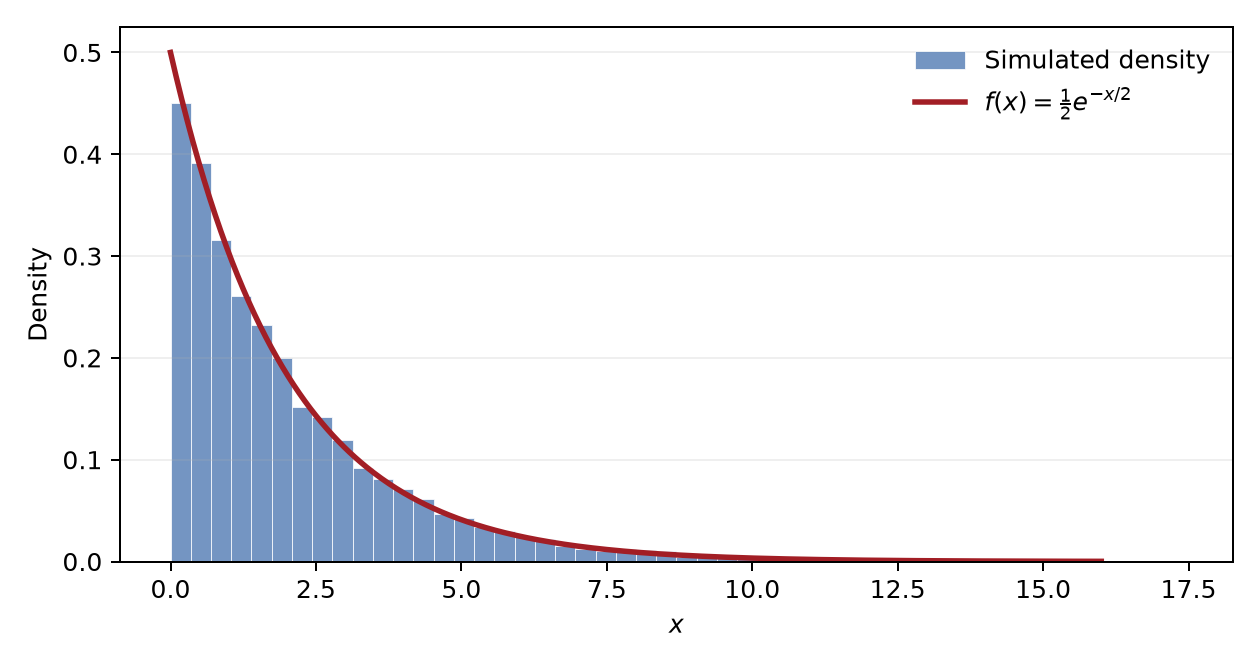
\includegraphics[width=0.70\textwidth]{q2_exponential.png}\end{center}
有限样本不会精确重现理论矩。应同时检查图形、均值和方差。

\section{第 3 题：接受--拒绝抽样}
目标密度 $f(x)=3x^2$，提议密度 $g(x)=2x$，定义域均为 $[0,1]$。按题目要求使用接受--拒绝法。

\subsection*{先理解候选样本}
若 $V\sim U(0,1)$、$X'=\sqrt V$，则 $P(X'\leq x)=P(V\leq x^2)=x^2$；求导后得到候选密度 $g(x)=2x$。

\subsection*{(a) 包络常数}
对 $x>0$，$f(x)/g(x)=3x/2$，所以
\[
\boxed{\alpha=\sup_{0<x\leq1}\frac{f(x)}{g(x)}=\frac32}.
\]
$x=0$ 时两密度均为零，包络不等式仍成立；不需要给 $0/0$ 赋值。

\subsection*{(b) 接受概率}
\[
\frac{f(X')}{\alpha g(X')}
=\frac{3(X')^2}{(3/2)(2X')}=X'.
\]
另生成与 $V$ 独立的 $U\sim U(0,1)$，接受条件就是 $\boxed{U\leq X'=\sqrt V}$。
\begin{idea}
\textbf{为什么筛选有效？} 在 $x$ 附近，候选密度乘接受概率为
$g(x)\,f(x)/[\alpha g(x)]=f(x)/\alpha$。总接受概率是 $\int f(x)/\alpha\,dx=1/\alpha$，所以条件于接受后的密度正是 $f(x)$。
\end{idea}

\subsection*{(c) 生成 $n$ 个接受样本的伪代码}
\begin{lstlisting}
accepted = []
proposals = 0
while len(accepted) < n:
    V = Uniform(0, 1)
    U = Uniform(0, 1)  # independent of V
    candidate = sqrt(V)
    proposals += 1
    if U <= candidate:
        accepted.append(candidate)
efficiency = n / proposals
\end{lstlisting}
停止条件是已接受 $n$ 个，不是只提议 $n$ 次。

\subsection*{(d) 模拟与直方图}
对 $10{,}000$ 个接受值画密度直方图，叠加 $f(x)=3x^2$。因为 $f$ 随 $x$ 增大，右侧样本较密。
\begin{center}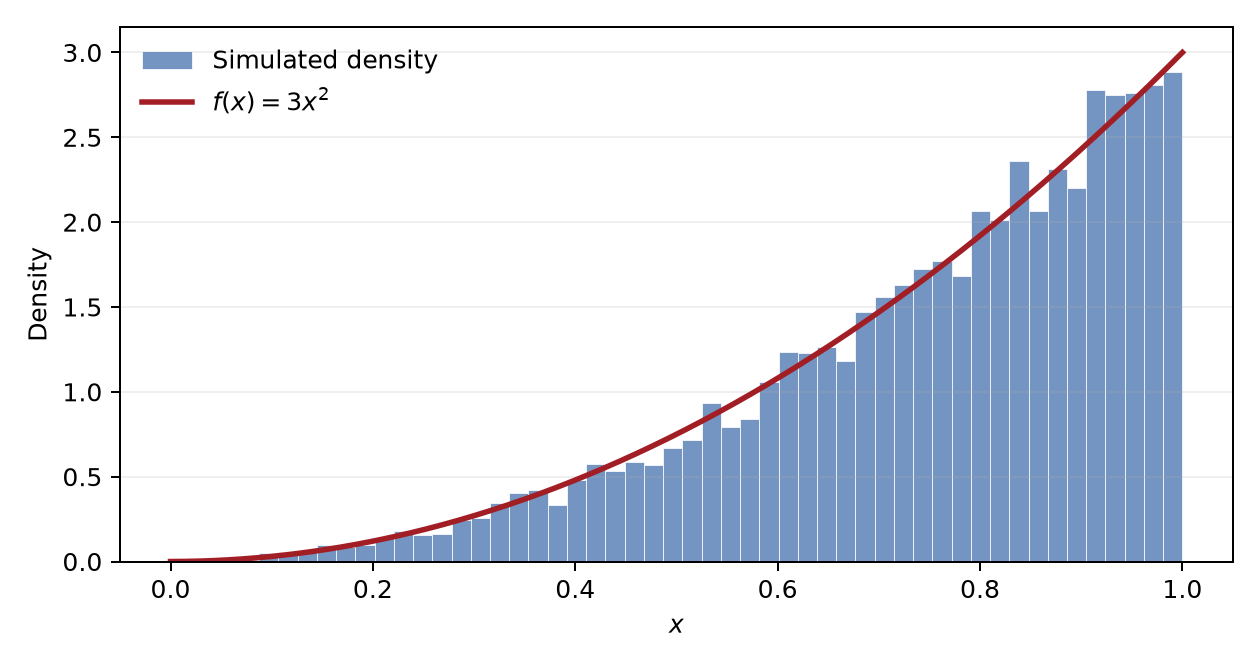
\includegraphics[width=0.70\textwidth]{q3_rejection.png}\end{center}

\subsection*{(e) 理论与经验效率}
理论接受率为 $1/\alpha=2/3$。接受 $10{,}000$ 个样本预计需约 $15{,}000$ 次提议。本次实际提议 \QThreeProposals{} 次，经验效率为 $10{,}000/\QThreeProposals=\QThreeEfficiency$，接近理论值。

\section{第 4 题：蒙特卡洛积分}
目标是 $I=\int_0^1e^{-x^2}\,dx$。

\subsection*{(a) 把积分写成期望}
若 $X\sim U(0,1)$，其密度在区间内为 $1$，故
\[
I=\int_0^1e^{-x^2}\cdot1\,dx=\E[e^{-X^2}],
\qquad
\boxed{\widehat I_N=\frac1N\sum_{i=1}^N e^{-X_i^2}}.
\]
这里的 $X_i$ 应独立。积分误差变成了样本平均的随机波动。

\subsection*{(b) 四个样本量}
对 $N=100,1{,}000,10{,}000,100{,}000$，分别平均前 $N$ 个值。参考值为
\[
I=\frac{\sqrt\pi}{2}\operatorname{erf}(1)\approx\QFourExact.
\]
样本估计不必随 $N$ 增大而单调靠近参考值。

\subsection*{(c) 样本标准差与区间}
对 $H_i=e^{-X_i^2}$，以
$s_H^2=(N-1)^{-1}\sum_i(H_i-\widehat I_N)^2$
计算样本方差，再用 $\widehat I_N\pm1.96s_H/\sqrt N$：
\begin{center}\small
\begin{tabular}{rrrrr}
\toprule
$N$&估计 $\widehat I_N$&样本标准差 $s_H$&95\% 下限&95\% 上限\\\midrule
100&\QFourAMean&\QFourASD&\QFourALow&\QFourAHigh\\
1,000&\QFourBMean&\QFourBSD&\QFourBLow&\QFourBHigh\\
10,000&\QFourCMean&\QFourCSD&\QFourCLow&\QFourCHigh\\
100,000&\QFourDMean&\QFourDSD&\QFourDLow&\QFourDHigh\\
\bottomrule
\end{tabular}\end{center}

\subsection*{(d) 区间宽度}
近似全宽为 $2(1.96)s_H/\sqrt N$。这里 $s_H$ 大致稳定在 $0.2$ 附近，所以 $N$ 乘 $10$，宽度约乘 $1/\sqrt{10}$；$N$ 乘 $100$，宽度约乘 $1/10$。

\section{第 5 题：普通蒙特卡洛期权定价}
在风险中性测度下，
\[
c_0=e^{-rT}\E[(S_T-K)^+],\quad
S_T=S_0\exp\!\left((r-\tfrac12\sigma^2)T+\sigma\sqrt T\,Z\right),
\quad Z\sim N(0,1).
\]
本题取 $S_0=95$、$K=100$、$r=0.01$、$\sigma=0.4$、$T=1$。

\subsection*{(a) 推导估计量}
每次独立抽 $Z_i$，计算
\[
S_T^{(i)}=95e^{-0.07+0.4Z_i},\quad
W_i=e^{-0.01}(S_T^{(i)}-100)^+,\quad
\boxed{\widehat c_N=\frac1N\sum_{i=1}^NW_i}.
\]
其中 $(x)^+=\max(x,0)$。使用贴现收益，是因为今天的价格等于未来风险中性收益的贴现期望。

\subsection*{(b) $10{,}000$ 条路径}
平均 $10{,}000$ 个 $W_i$，本次得到 \QFiveAMean。这是随机估计，不是解析价格。

\subsection*{(c) 第一次模拟的置信区间}
若 $s_W$ 为贴现收益的样本标准差，则估计标准误差为 $s_W/\sqrt N$，区间为 $\widehat c_N\pm1.96s_W/\sqrt N$。本次 $s_W=\QFiveASD$、标准误差 \QFiveASE、区间 $[\QFiveALow,\QFiveAHigh]$。

\subsection*{(d) $100{,}000$ 条路径}
\begin{center}\small
\begin{tabular}{rrrrr}
\toprule
$N$&价格估计&估计标准误差&95\% 下限&95\% 上限\\\midrule
10,000&\QFiveAMean&\QFiveASE&\QFiveALow&\QFiveAHigh\\
100,000&\QFiveBMean&\QFiveBSE&\QFiveBLow&\QFiveBHigh\\
\bottomrule
\end{tabular}\end{center}
第二行的区间更窄。Black--Scholes 解析价格约为 \QFiveExact，可用来核对；样本更多不保证单次估计必定更接近它。

\subsection*{(e) 样本量与标准误差}
由于 $\SE(\widehat c_N)=\sigma_W/\sqrt N$，将样本数增至 $100N$ 只会使标准误差约变为原来的 $1/10$。
\begin{pitfall}
作业 (b) 与 (d) 实际从 $10{,}000$ 增至 $100{,}000$，只增加 $10$ 倍；(e) 单独问一般的 $100$ 倍情形。比较表格两行时，预期标准误差因子是 $1/\sqrt{10}$。
\end{pitfall}

\section{第 6 题：反变量法}
这一题仍估计看涨期权价格，但每个正态数 $Z_i$ 与 $-Z_i$ 配成一对。

\subsection*{(a) 为什么同分布}
标准正态密度 $\phi(z)=(2\pi)^{-1/2}e^{-z^2/2}$ 满足 $\phi(-z)=\phi(z)$，故 $Z$ 与 $-Z$ 同分布。配对路径分别有正确的边缘分布，但同一对内部并不独立。

\subsection*{(b) $10{,}000$ 对如何计算}
\[
S_{T,i}^{\pm}=95e^{-0.07\pm0.4Z_i},\qquad
A_i=\frac{e^{-0.01}}2
\left[(S_{T,i}^{+}-100)^++(S_{T,i}^{-}-100)^+\right],
\qquad
\widehat c_{\rm AV}=\frac1N\sum_{i=1}^N A_i.
\]
先把每一对收益平均为一个 $A_i$，再平均 $10{,}000$ 个 $A_i$。不同配对之间独立，每对的期望仍是 $c_0$。

\subsection*{(c) 价格与区间}
以 $10{,}000$ 个 $A_i$ 的样本标准差 $s_A$ 计算标准误差 $s_A/\sqrt{10{,}000}$。本次价格为 \QSixAVMean，$s_A=\QSixAVSD$，标准误差为 \QSixAVSE，近似 $95\%$ 区间为 $[\QSixAVLow,\QSixAVHigh]$。
\begin{pitfall}
虽然计算了 $20{,}000$ 个单边收益，同一对的两项相关。不能将它们当作 $20{,}000$ 个独立样本来计算区间。
\end{pitfall}

\subsection*{(d) 为什么标准误差较小}
若一对贴现收益为 $P^+,P^-$，各自方差为 $\sigma_P^2$、相关系数为 $\rho$，则
\[
\Var\!\left(\frac{P^++P^-}{2}\right)
=\frac{\sigma_P^2}{2}(1+\rho).
\]
$P^+$ 随 $Z$ 不减，$P^-$ 随 $Z$ 不增，因此 $\rho\leq0$，配对平均值的方差较小。
\begin{center}\small
\begin{tabular}{lrr}
\toprule
方法&价格估计&估计标准误差\\\midrule
Q5：10,000 条普通路径&\QFiveAMean&\QFiveASE\\
Q6：同一组 $Z_i$ 的普通路径&\QSixCrudeMean&\QSixCrudeSE\\
Q6：10,000 对反变量&\QSixAVMean&\QSixAVSE\\
\bottomrule
\end{tabular}\end{center}
反变量标准误差较小。一对计算两次收益；严格比较相同计算量时，还应与 $20{,}000$ 条独立普通路径比较。较小的标准误差不保证某一次点估计恰好更接近真值。

\section{第 7 题：控制变量法}
目标为 $\theta=\E[X^{0.9}]$，其中 $X\sim\operatorname{Exp}(1)$。令 $H=X^{0.9}$，选 $Y=X$ 作控制变量，因为它与 $H$ 高度相关，且 $\E[Y]=1$ 已知。

\subsection*{(a) 生成样本}
对 $i=1,\ldots,10{,}000$，生成独立 $U_i\sim U(0,1)$，令 $X_i=-\ln(1-U_i)$。与第 2 题不同，这里的指数均值为 $1$。

\subsection*{(b) 普通估计}
令 $H_i=X_i^{0.9}$，则 $\widehat\theta_{\rm crude}=N^{-1}\sum_iH_i$。本次结果是 \QSevenCrudeMean。解析参考值为 $\E[X^{0.9}]=\Gamma(1.9)\approx\QSevenExact$。

\subsection*{(c) 求样本最佳系数}
令 $H^*=H+c(X-1)$。固定 $c$ 时，$\E[H^*]=\E[H]$，因为 $\E[X-1]=0$。展开方差：
\[
\Var(H^*)=\Var(H)+2c\Cov(H,X)+c^2\Var(X).
\]
对此二次式求最小值，得到
\[
\boxed{c^*=-\frac{\Cov(H,X)}{\Var(X)}},\qquad
\widehat c
=-\frac{\sum_i(H_i-\bar H)(X_i-\bar X)}
        {\sum_i(X_i-\bar X)^2}
=\QSevenCoeff.
\]
样本协方差与样本方差的 $1/(N-1)$ 因子会相消。负系数抵消二者共同上涨的波动。

\subsection*{(d) 构造控制变量估计}
对同一批样本逐个计算
\[
H_i^*=X_i^{0.9}+\widehat c(X_i-1),\qquad
\widehat\theta_{\rm CV}=\frac1N\sum_iH_i^*.
\]
本次结果为 \QSevenCVMean，接近参考值 \QSevenExact。

\subsection*{(e) 比较标准差}
\begin{center}\small
\begin{tabular}{lrrr}
\toprule
方法&均值估计&样本值标准差&均值估计标准误差\\\midrule
普通 $H_i$&\QSevenCrudeMean&\QSevenCrudeSD&\QSevenCrudeSE\\
控制变量 $H_i^*$&\QSevenCVMean&\QSevenCVSD&\QSevenCVSE\\
\bottomrule
\end{tabular}\end{center}
作业直接要求比较的是样本值标准差 \QSevenCrudeSD{} 与 \QSevenCVSD；各除以 $\sqrt{10{,}000}=100$ 才得到均值的估计标准误差。

还可解析核对系数。对 $X\sim\operatorname{Exp}(1)$，$\E[X^p]=\Gamma(p+1)$，因此
\[
\Cov(X^{0.9},X)=\Gamma(2.9)-\Gamma(1.9)
=0.9\Gamma(1.9),\quad \Var(X)=1,
\]
即 $c^*=-0.9\Gamma(1.9)\approx\QSevenExactCoeff$。由同一批数据估计 $\widehat c$ 时，固定 $c$ 的精确无偏性在有限样本下不能原样照搬；这里最重要的是明显的方差缩减。

\section{把七道题连起来}
\begin{center}
\begin{tabular}{p{25mm}p{110mm}}
\toprule
题目&核心问题\\\midrule
1--3&如何获得指定分布的样本：伪随机数、逆变换、接受--拒绝。\\
4--5&如何把积分或价格变成期望，并用样本平均和置信区间估计。\\
6--7&如何保持目标期望，同时降低估计量的方差。\\
\bottomrule
\end{tabular}
\end{center}

\section*{资料与复现}
\addcontentsline{toc}{section}{资料与复现}
题目依据 \texttt{MATH4907\_2026Sem1\_A5.pdf}，课程概念参照 \texttt{MonteCarlo.beamer-2.pdf}。同目录的 \texttt{05\_tutorial.py} 生成数值和图，\texttt{05\_results.tex} 保存数值宏；使用按题目分开的固定随机种子。

\end{document}
